% Copyright 2006 by Till Tantau
%
% This file may be distributed and/or modified
%
% 1. under the LaTeX Project Public License and/or
% 2. under the GNU Free Documentation License.
%
% See the file doc/generic/pgf/licenses/LICENSE for more details.

\section{To Path Library}

\label{library-to-paths}

\begin{tikzlibrary}{topaths}
  This library provides predefined to paths for use with the |to|
  path operation. After loading this package, you can say for instance
  |to [loop]| to add a loop to a node.

  This library is loaded automatically by \tikzname, so you do not
  need to load it yourself.
\end{tikzlibrary}


\subsection{Straight Lines}

The following style installs a to path that is simply a straight line
from the start coordinate to the target coordinate.

\begin{key}{/tikz/line to}
  Causes a straight line to be added to the path upon a |to| or an
  |edge| operation.
\begin{codeexample}[]
\tikz {\draw (0,0) to[line to] (1,0);}
\end{codeexample}
\end{key}


\subsection{Curves}

The |curve to| style causes the to path to be set to a curve. The
exact way this curve looks can be influenced via a number of options.

\begin{key}{/tikz/curve to}
  Specifies that the |to path| should be a curve. This curve will
  leave the start coordinate at a certain angle, which can be
  specified using the |out| option. It reaches the target coordinate
  also at a certain angle, which is specified using the |in|
  option. The control points of the curve are at a certain distance
  that is computed in different ways, depending on which options are
  set.

  All of the following options implictly cause the |curve to| style to
  be installed.

  \begin{key}{/tikz/out=\meta{angle}}
    The angle at which the curve leaves the start coordinate. If the
    start coordinate is a node, the start coordinate is the point on the
    border of the node at the given \meta{angle}. The control point
    will, thus, lie at a certain distance in the direction \meta{angle}
    from the start coordinate.
\begin{codeexample}[]
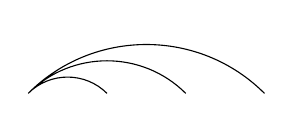
\begin{tikzpicture}[out=45,in=135]
  \draw (0,0) to (1,0)
        (0,0) to (2,0)
        (0,0) to (3,0);
\end{tikzpicture}
\end{codeexample}
  \end{key}
  \begin{key}{/tikz/in=\meta{angle}}
    The angle at which the curve reaches the target coordinate.
  \end{key}

  \begin{key}{/tikz/relative=\meta{true or false} (default true)}
    This option tells \tikzname\ whether the |in| and |out| angles
    should be considered absolute or relative. Absolute means that an
    |out| angle of 30$^\circ$ means that the curve leaves the start
    coordinate at an angle of 30$^\circ$ relative to the paper (unless,
    of course, further transformations have been installed). A
    \emph{relative} angle is, by comparison, measured relative to a
    straight line from the start coordinate to the target
    coordinate. Thus, a relative angle of 30$^\circ$ means that the
    curve will bend to the left from the line going straight from the
    start to the target. For the target, the relative coordinate is
    measured in the same manner, namely relative to the line going from
    the start to the target. Thus, an angle of 150$^\circ$ means that
    the curve will reach target coming slightly from the left.

\begin{codeexample}[]
\begin{tikzpicture}[out=45,in=135,relative]
  \draw (0,0) to (1,0)
              to (2,1)
              to (2,2);
\end{tikzpicture}
\end{codeexample}

\begin{codeexample}[]
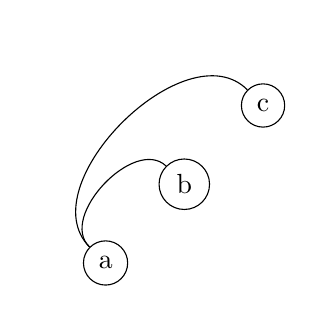
\begin{tikzpicture}[out=90,in=90,relative]
  \node [circle,draw] (a) at (0,0) {a};
  \node [circle,draw] (b) at (1,1) {b};
  \node [circle,draw] (c) at (2,2) {c};

  \path (a) edge (b)
            edge (c);
\end{tikzpicture}
\end{codeexample}
  \end{key}

  \begin{key}{/tikz/bend left=\meta{angle} (default \normalfont last value)}
    This option sets |out=|\meta{angle}|,in=|$180-\meta{angle}$|,relative|. If no
    \meta{angle} is given, the last given |bend left| or |bend right|
    angle is used.  
  
\begin{codeexample}[]
\begin{tikzpicture}[shorten >=1pt,node distance=2cm,on grid]
  \node[state,initial]  (q_0)                {$q_0$};
  \node[state]          (q_1) [right=of q_0] {$q_1$};
  \node[state,accepting](q_2) [right=of q_1] {$q_2$};

  \path[->] (q_0) edge              node [above]  {0} (q_1)
                  edge [loop above] node          {1} ()
                  edge [bend left]  node [above]  {1} (q_2)
                  edge [bend right] node [below]  {0} (q_2)
            (q_1) edge              node [above]  {1} (q_2);
\end{tikzpicture}
\end{codeexample}

\begin{codeexample}[]
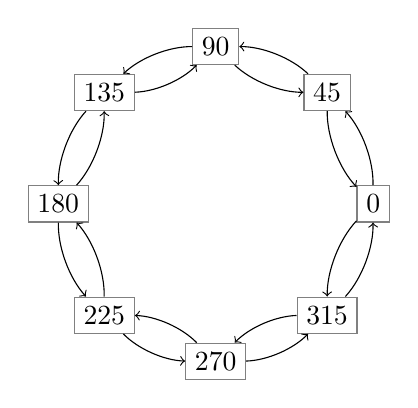
\begin{tikzpicture}
  \foreach \angle in {0,45,...,315}
    \node[rectangle,draw=black!50] (\angle) at (\angle:2) {\angle};

  \foreach \from/\to in {0/45,45/90,90/135,135/180,
                         180/225,225/270,270/315,315/0}
    \path (\from) edge [->,bend right=22,looseness=0.8] (\to)
                  edge [<-,bend left=22,looseness=0.8] (\to);
\end{tikzpicture}
\end{codeexample}
  \end{key}

  \begin{key}{/tikz/bend right=\meta{angle} (default \normalfont last  value)}
    Works like the |bend left| option, only the bend is to the other side.
  \end{key}

  \begin{key}{/tikz/bend angle=\meta{angle}}
    Sets the angle to be used by the |bend left| or |bend right|, but
    without actually selecting the |curve to| or the |relative|
    option. This is useful for globally specifying a |bend angle| for a
    whole picture.
  \end{key}

  \begin{key}{/tikz/looseness=\meta{number} (initially 1)}
    This number specifies how ``loose'' the curve will be. In detail,
    the following happens: \tikzname\ computes the distance between the
    start and the target coordinate (if the start and/or target
    coordinate are nodes, the distance is computed between the points on
    their border). This distance is then multiplied by a fixed factor
    and also by the factor \meta{number}. The resulting distance, let us
    call it $d$, is then used as the distance of the control points from
    the start and target coordinates.

    The fixed factor has been chosen in such a way that if \meta{number}
    is |1|, if the |in| and |out| angles differ by
    90$\circ$, then a quarter circle results:
  \begin{codeexample}[]
\tikz \draw (0,0) to [out=0,in=-90]               (1,1);
\tikz \draw (0,0) to [out=0,in=-90,looseness=0.5] (1,1);
  \end{codeexample}
  \end{key}

  \begin{key}{/tikz/out looseness=\meta{number}}
    specifies the looseness factor for the out distance only.
  \end{key}

  \begin{key}{/tikz/in looseness=\meta{number}}
    specifies the looseness factor for the in distance only.
  \end{key}
  \begin{key}{/tikz/min distance=\meta{distance}}
    If the computed distance for the start and target coordinates are
    below \meta{distance}, then \meta{distance} is used instead.
  \end{key}
  \begin{key}{/tikz/max distance=\meta{distance}}
    If the computed distance for the start and target coordinates are
    above \meta{distance}, then \meta{distance} is used instead.
  \end{key}
  \begin{key}{/tikz/out min distance=\meta{distance}}
    The mininimum distance set only for the start coordinate.
  \end{key}
  \begin{key}{/tikz/out max distance=\meta{distance}}
    The maximum distance set only for the start coordinate.
  \end{key}
  \begin{key}{/tikz/in min distance=\meta{distance}}
    The min distance set only for the target coordinate.
  \end{key}
  \begin{key}{/tikz/in max distance=\meta{distance}}
    The max distance set only for the target coordinate.
  \end{key}
  \begin{key}{/tikz/distance=\meta{distance}}
    Set the min and max distance to the same value \meta{distance}. Note
    that this causes any computed distance $d$ to be ignored and
    \meta{distance} to be used instead.
\begin{codeexample}[]
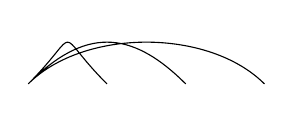
\begin{tikzpicture}[out=45,in=135,distance=1cm]
  \draw (0,0) to (1,0)
        (0,0) to (2,0)
        (0,0) to (3,0);
\end{tikzpicture}
\end{codeexample}
  \end{key}
  \begin{key}{/tikz/out distance=\meta{distance}}
    Sets the min and max out distance.
  \end{key}
  \begin{key}{/tikz/in distance=\meta{distance}}
    Sets the min and max in distance.
  \end{key}
  \begin{key}{/tikz/out control=\meta{coordinate}}
    This option causes the \meta{coordinate} to be used as the start
    control point. All computations of $d$ are ignored. You can use a
    coordinate like |+(1,0)| to specify a point relative to the start
    coordinate.
  \end{key}
  \begin{key}{/tikz/in control=\meta{coordinate}}
    This option causes the \meta{coordinate} to be used as the target
    control point.
  \end{key}
  \begin{key}{/tikz/controls=\meta{coordinate}| and |\meta{coordinate}}
    This option causes the \meta{coordinate}s to be used as control
    points. 
\begin{codeexample}[]
\tikz \draw (0,0) to [controls=+(90:1) and +(90:1)] (3,0);
\end{codeexample}
  \end{key}
\end{key}


\subsection{Loops}

\begin{key}{/tikz/loop}
  This key is similar to the |curve to| key, but differs in the
  following ways: First, the actual target coordinate is ignored and the
  start coordiante is used as the target coordinate. Thus, it is
  allowed not to provide any target coordinate, which can be useful
  with unnamed nodes. Second, the |looseness| is set to |8| and the
  |min distance| to |5mm|. These settings result in rather nice loops
  when the opening angle (difference between |in| and |out|) is
  30$^\circ$.
\begin{codeexample}[]
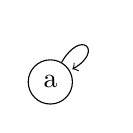
\begin{tikzpicture}
  \node [circle,draw] {a} edge [in=30,out=60,loop] ();    
\end{tikzpicture}
\end{codeexample}
\end{key}

\begin{stylekey}{/tikz/loop above}
  Sets the |loop| style and sets in and out angles such that
  loop is above the node. Furthermore, the |above| option is set,
  which causes a node label to be placed at the correct position. 
\begin{codeexample}[]
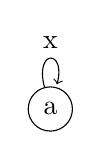
\begin{tikzpicture}
  \node [circle,draw] {a} edge [loop above] node {x} ();    
\end{tikzpicture}
\end{codeexample}
\end{stylekey}
\begin{stylekey}{/tikz/loop below} Works like the previous option. \end{stylekey}
\begin{stylekey}{/tikz/loop left} Works like the previous option. \end{stylekey}
\begin{stylekey}{/tikz/loop right} Works like the previous option. \end{stylekey}
\begin{stylekey}{/tikz/every loop (initially {->,shorten >=1pt})}
  This style is installed at the beginning of
  every loop.
\begin{codeexample}[]
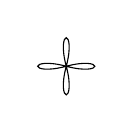
\begin{tikzpicture}[every loop/.style={}]
  \draw (0,0) to [loop above] () to [loop right] ()
              to [loop below] () to [loop left]  ();
\end{tikzpicture}
\end{codeexample}
\end{stylekey}



%%% Local Variables: 
%%% mode: latex
%%% TeX-master: "pgfmanual-pdftex-version"
%%% End: 
